% Muster für die Seminarausarbeitung
% HPI Potsdam

\documentclass[11pt, a4paper]{article}

\usepackage[english]{babel}
\usepackage[utf8]{inputenc} %Korrekte Kodierung der Umlaute nach UTF-8
\usepackage[T1]{fontenc} %Korrekte Kodierung der Umlaute nach UTF-8
\usepackage{makeidx} %Zur automatischen Indexerstellung
\usepackage{amsfonts}
\usepackage{mathtools}
\usepackage{amssymb}
\usepackage{epsfig}   % Zum Einbinden von Bildern
\usepackage{url}      % Korrekter Satz von URLs
\usepackage{color}    % Verwendung von Farben
\usepackage{listings} % Korrekter Satz von Listings und Quellcode
\usepackage[parfill]{parskip}

%Hilfs-Fonts - ohne Serifen (hier für Tabellen)
\newfont{\bib}{cmss8 scaled 1040}
%\newfont{\bibf}{cmssbx8 scaled 1040}

\definecolor{lightgray}{gray}{0.85}
\DeclareMathOperator*{\argmax}{\arg\!\max}
\DeclarePairedDelimiterX\Set[2]{\lbrace}{\rbrace}%
 { #1 \,\delimsize|\, #2 }
 \numberwithin{equation}{section}

%Seitenformat-Definitionen
\topmargin0mm
\textwidth147mm
\textheight214mm
\evensidemargin5mm
\oddsidemargin5mm
\footskip19mm
\parindent=0in

\makeindex % legt das Index-File an


\begin{document}

\begin{titlepage}
  \begin{center}
    \mbox{}
    \vspace{1cm}

    {\huge Match Forrest, Match! \\[1em] {\LARGE Creating a unified dataset of Movies}}

    \vspace{4cm}

    Seminar paper for \\[1em]
    {\large \sc Semantic Multimedia 2014 - A LOD of Movies} \\[1em]
    Summer Semester 2014 \\[1em]
    Hasso-Plattner-Institut for Softwaresystemtechnik GmbH \\[1em]
    University Potsdam

    \vspace{3cm}

		Authors:

    \vspace{1em}

		{\Large Tanja Bergmann} \\
		{\Large Stefan Bunk} \\
		{\Large Tim Draeger} \\
		{\Large Dominik Müller} \\
		{\Large Ricarda Schüler}

    \vspace{3em}

    August 19th, 2014
  \end{center}
\end{titlepage}


\setcounter{page}{1}

% Zweite Seite = Kurzzusammenfassung
\begin{abstract}
\noindent

TODO
Tim, Tanja, Stefan

\bigskip

\end{abstract}


\newpage

% Dritte Seite = Inhaltsverzeichnis
\tableofcontents

\newpage

\section{Introduction}
\label{sec_introduction}



\newpage
\section{Related Work}
\label{sec_related_work}


Triplification (http://linkedmdb.org/), Referenz zur Triplification http://triplify.org/Challenge/ von Movies\\\\

Hassanzadeh and Consens tried in \cite{LMDB} to unify multiple sources of movie data (among them IMDb and Freebase) into an open linked data set.
They utilize approximate string matching methods on movies' titles to find sameAs relation between movies of different sources.
Hassanzadeh and Consens measured the accuracy of their method when using edit similarity, Jaccard or WeightedJaccard, as well as other measures used in information retrieval for string matching.\\\\

Leveraging Usage Data for Linked Data Movie Entity Summarization 
\cite{MovieSummarization}
%http://arxiv.org/pdf/1204.2718v1.pdf

T. Berners-Lee. Linked Data, Design Issues.
\url{http://www.w3.org/DesignIssues/LinkedData.html}, 27 July 2006.
\newpage
\section{Method}
\label{sec_method}

... some text ...

\subsection{Data Sources}
\label{subsec_method_datasources}
\subsection{Ontology}
\label{subsec_method_ontology}

As described in the previous section, different data sources with different data formats were used. 
To create a unified dataset and therefore enable simple querying over all data, a unified ontology was defined.


The following resources, defined by the dataset, were used in the system. 
In most cases a corresponding dbpedia entity exists and thus was used.
If no dbpedia entity was present, freebase entities or newly defined ones were used.

\begin{itemize}
\item Movie: dbpedia-owl:Film
\item Award: dbpedia-owl:Award
\item MoviePerson: dbpedia-owl:Person
\item Character: freebase:film/performance
\item Aka (also known as): aka
\item ReleaseInfo: releaseInfo

\end{itemize}

A MoviePerson can have multiple sub-types of dbpedia-owl:Person, depending on the jobs the person had in any movies they worked on. 
As shown in Figure \ref{fig_ontology} a distinction between e.g. director, writer, producer was made.
Relations between the listed resources are also shown in Figure \ref{fig_ontology}.

%dbpedia-owl:Actor,
%dbpedia-owl:director,
%dbpedia-owl:Writer,
%dbpedia-owl:producer,
%dbpedia-owl:coProducer,
%dbpedia-owl:makeUpArtist,
%dbpedia-owl:costumeDesigner,
%dbpedia-owl:specialEffects,
%dbpedia-owl:setDesigner,
%dbpedia-owl:storyEditor


\begin{figure}[h!]
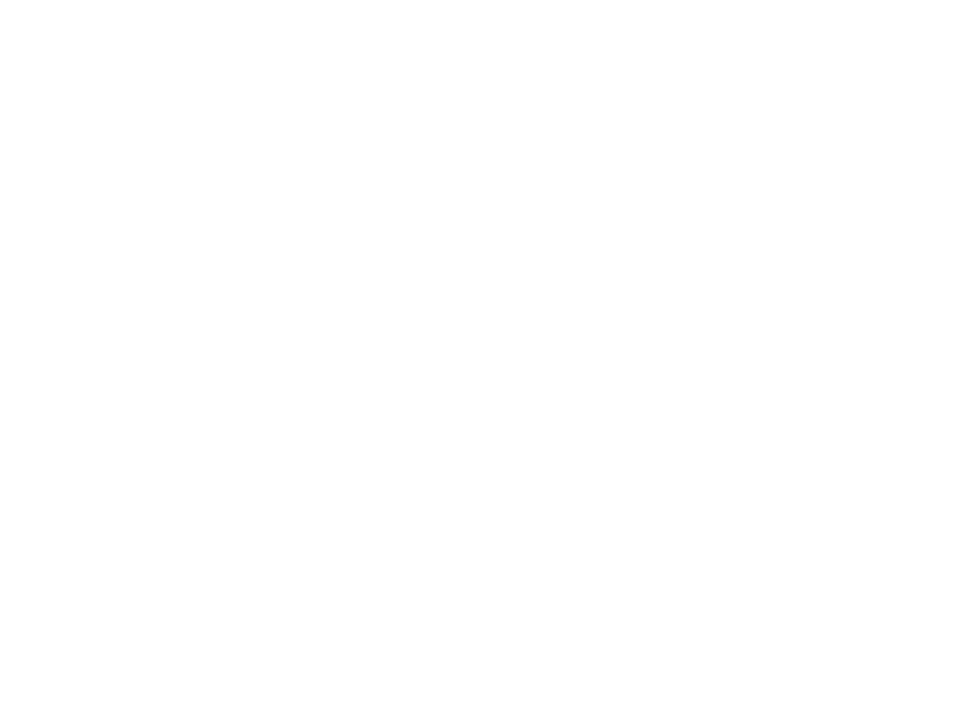
\includegraphics[width=\textwidth]{images/ontology.pdf}
\caption{Ontology}
\label{fig_ontology}
\end{figure}

The naive way to express roles, shown in Figure \ref{fig_ontology}, was one \emph{character} class which was connected to the corresponding movie (via film/performance) and actor (actor or performance).
This meant that a role which exists in multiple movies (e.g. "cleaning lady") would be one resource with an \emph{actor} property for each actor who had ever portrayed this role. 

This approach could cause problems in some cases.
One such case is an actor who played a certain role in an old movie but also appears in the movie's newer remake.
In the remake, they might play a different role while another actor plays their original role. 
An example for this is the movie "Starsky \& Hutch" (2004), which is a remake of the (1970s) television series with the same name.
In the movie, both actors which originally portrayed Starsky and Hutch get a cameo appearance alongside the new cast for their old roles.
With the naive approach, the system could not know who played the Starsky role in the remake, because only references to the movies and the actors are given.

Therefore, an additional class of \emph{MovieCharacter} was introduced.
The resources of this class knows exactly one movie and all actors who played this role in this one movie.
The \emph{MovieCharacter} has a connection, named \emph{Character}, to the \emph{Character} class, which describes the general role.
This means that the \emph{MovieCharacter} in the "Starsky \& Hutch" example is "StarksyStarsky\&Hutch1970" and the \emph{Character} is "Starksy".

%TODO ??More detailed description of diagram??
%TODO ??How many total different entity types, relation types, property types??
\subsection{Architecture}
\label{subsec_method_architecture}

The architecture of \emph{Match Forrest, Match!} is shown in Figure \ref{fig_architecture}.
\\ \\
The central component of the system is the \textit{Task Distributor}.
This component is responsible for managing the other components, \textit{Crawler}, \textit{Triplifier}, \textit{Updater} and \textit{Matcher and Merger}.
The details of this messaging systems are explained in Section \ref{subsubsec_messaging_infrastructure}.
\\ \\
In general, the first step to get a movie into the system is to get the acutal movie resource.
This step is executed by the \textit{Crawler.}
This component is responsible for downloading websites and for sending requests to the provided API from a data source.

Once the page is downloaded, the \textit{Triplifier} can triplify the resource.
This means it extracting the information from the resource and creating triples out of it.
Therefore the ontology, defined in Section \ref{subsec_method_ontology}, is used.

The component \textit{Matcher and Merger} is in charge of matching two movies from different data sources, so they only can be found once in the resulting dataset.
This component is explained in detail in Section \ref{subsec_method_matching}.

The updater, described in Section \ref{subsec_method_updating}, ensures that the movies are always up to date.
\\ \\
The triplestore \textit{Virtuoso} is used to store the resulting triples.
To distinguish between the sources of the different triples, triples from each data source are stored in the graph named after the source.
Thus, there are four graphs in the triplestore, \textit{IMDb}, \textit{Freebase}, \textit{TMDb} and \textit{OFDb}.

\begin{figure}[ht]
  \begin{center}
  \includegraphics[width=0.5\textwidth]{images/architecture.pdf}
  \end{center}
  \caption{Architecture}
  \label{fig_architecture}
\end{figure}

\subsubsection{Messaging Infrastructure}
\label{subsubsec_messaging_infrastructure}

... TODO ...
%TODO

\begin{figure}[ht]
  \begin{center}
  \includegraphics[width=0.5\textwidth]{images/rabbit_mq.pdf}
  \end{center}
  \caption{Messaging Infrastructure using RabbitMQ}
  \label{fig_messaging_infrastructure}
\end{figure}
%!TEX root = ../../lod-group1.tex
\subsection{Triplification of Movie Resources}
\label{subsec_method_triplification}

Triplification is the step of converting information from a movie resource into triples.
The triples are created according to the ontology, defined in Section~\ref{subsec_method_ontology}.

To create triples from the raw file of the movie resource, the information in the file has to be mapped to a corresponding predicate.
For example, the title of the movie ``Forrest Gump'', displayed on a website, has to be converted into the triple
\begin{center}\emph{<http://movie/Forrest\_Gump> dbpprop:title ``Forrest Gump''}.\end{center}
To guarantee this, every data source was analyzed and parsed manually.
In this way, it is strictly defined, which part of a movie resource contains valuable information and which RDF predicate corresponds to the type of information.
\subsection{Matching}
\label{subsec_method_matching}

The following sections show the approach for matching (i.e. finding the same entity in different datasets) and merging (i.e. integrating two different datasets about the same entity into one.)

\subsubsection{Problem statement}
After loading the initial dataset into the database, the task is to integrate other datasets to create a whole dataset with more information than a single one can provide on their own.
% TODO: Why IMDB?
However, simply dumping the second dataset into the database would lead to duplicated entries and thereby decreasing the overall quality of the database.
Thus, the datasets need to be aggregated and unified by looking for a match for each new entry in the old dataset.
Potentially, this has to be done for matching every entry, such as movies, actors, characters and more but the next parts focus on matching just movies to each other.

A first approach is to match movies only by their name.
However, only using the name as a matching criteria yields multiple problems, such as:
\begin{itemize}
	\item different movies having the same name e.g.
	\begin{itemize} 
        \item The Avengers (2012) vs. The Avengers (1998)
        \item Casino Royale (1967) vs. Casino Royale (2006)
    \end{itemize}
	\item same movies having different names in different datasets e.g.
	\begin{itemize} 
        \item Spelling errors: Batman vs Badman
        \item Localization: The Internship vs. Prakti.com
        \item Formatting: The Italian Job vs. Italian Job, The
     \end{itemize}
\end{itemize}
Hence, a more sophisticated approach needs to be developed to increase the quality of the dataset.

\subsubsection{Matching using actor overlap}
In general, the matching algorithm must satisfy two requirements:
\begin{enumerate}
	\item{High precision:} A movies should not be matched to a wrong movie, as this decreases the quality of the dataset. We want to find many matches, but it is important not to add too many wrong matches.
	\item{Performance:} With thousand of movies in each new dataset, matching should not take too long, as there are thousands of movies to match (e.g. TMDB has ca. 170,000 (TODO Check this number) movies to match.
	If each movie takes just 1 minute to match, the whole process for TMDB already takes $170,000~movies * 1 \frac{minute}{movie} * \frac{1}{1440} \frac{days}{minute} \approx 118~days$.
	This is just one data source, and only the current set of movies (remember, there are new movies every day from all data sources, which need to be merged)).
\end{enumerate}

This leads to two consequences: First, a certain level of confidence needs to be reached to match two movies to each other. Otherwise, it is impossible to detect movies, which are not matchable, because they are not in the database.
Second, comparing each movie with all movies in the database is not feasible.

This paper proposes the idea to first find a small list of movies that could be a match (henceforth called candidates) and then calculate a score for each of these candidates, which is based on the actors . Details are described in the following paragraphs.

Figure \ref{fig_matching_general} shows the general matching procedure:
First, we pass through each new movie, that we want to match.
For each movie $n_i \in N$ ($N$ is the set of movies we still need to match), we first select a small set of movies $C_{i}$ that could be a match (henceforth called candidates).
Then we calculate a score, which captures the similarity between $n_i$ and each $m_j \in C_i$.
This score is mostly based on the actor information we have about the two movies.
Finally, we choose the movie with the highest score, if the score is above a certain threshold.

\begin{figure}[ht]
  \begin{center}
  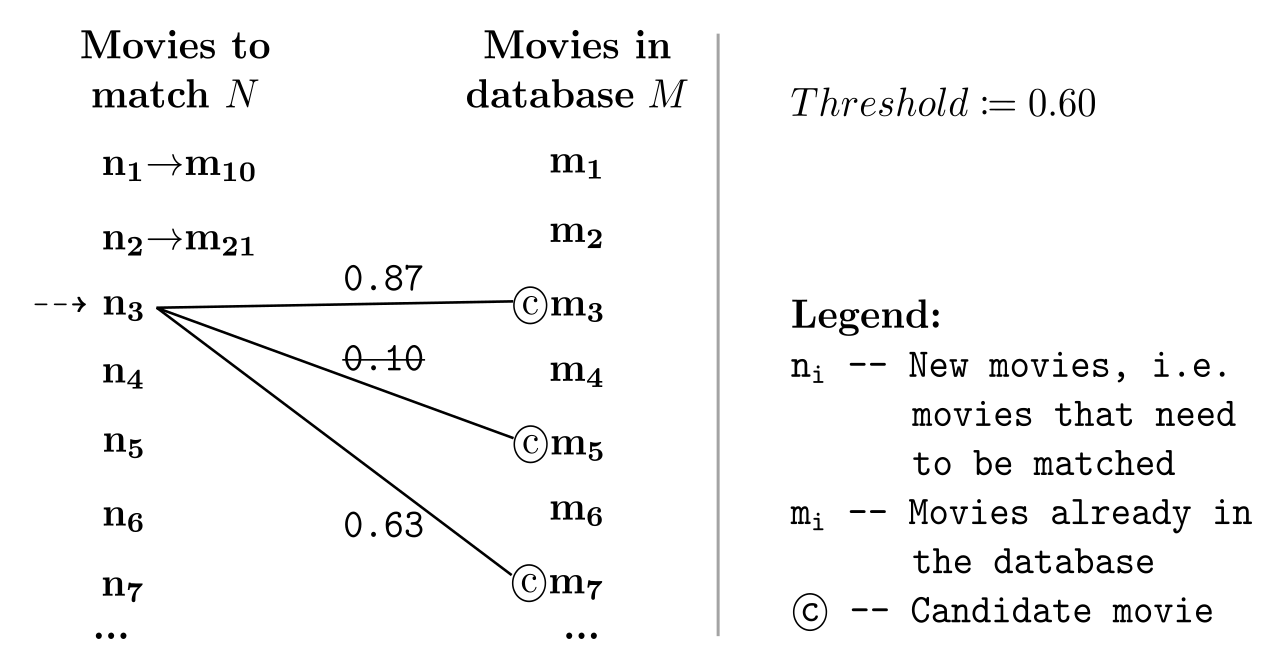
\includegraphics[width=0.8\textwidth]{images/matching_general.pdf}
  \end{center}
  \caption{This shows the general matching procedure. In this case, we would choose movie $m_3$ as a match for $n_3$, because it has the highest score and is above the threshold.}
  \label{fig_matching_general}
\end{figure}

The next paragraphs describe candidate selection and score calculation in detail.

\paragraph{Candidate selection}

The general goal of candidate selection is to reduce the set of all movies in the database to a smaller set of candidates.
There are two constraints working against each other:
\begin{itemize}
	\item The candidate should be as small as possible. This leads to fewer comparisions and thereby increased performance.
	\item The correct movie, i.e. the movie that needs to be matched to our current movie, must be in the candidate set, if it exists in the database.
\end{itemize}
The former would be optimized by returning nothing, the latter by returning everything, so a viable tradeoff has to be found.

The algorithm presented in this paper TODO Dominik.

\paragraph{Score calculation}
After the candidates have been selected, the next step is to find the best match.
For that, we use the actor information we have about $n_i$ and each $m_j$ in $C_i$.
Given
\begin{description}
	\item[$n_i$] the movie we want to match,
	\item[$C_i$] the set of candidates for the movie,
	\item[$A(movie)$] a function, which returns the actor names from a movie in one of our datasets,
	\item[$levenshtein(s_1, s_2)$] a function, which returns the edit distance (insert, remove, replace) between two strings.
\end{description}
we determine the best match as follows:

\begin{align}
	% \label{actor_overlap}
	best\_match(n_i) &= \argmax_{m_j \in C_i} score(n_i, m_j)\label{aoeq:1}\\
	score(n, m) &= \frac
	{\left\lvert  overlap\_set(A(n), A(m)) \right\rvert}
	{\left\lvert  A_{n} \right\rvert}\label{aoeq:2}\\
	overlap\_set(A_n, A_m) &= \Set*{a_n \in A_n}{\exists a_m \in A_m: levenshtein(a_n, a_m) < T},\label{aoeq:3} 
\end{align}
% \begin{equation}
% 	% \label{actor_overlap}
% 	be\_mh(n_i) = \argmax_{m_j \in C_i} sco(n_i, m_j)\label{aoeq:1}\\
% \end{equation}
where $T$ is a certain threshold parameter, that determines from which levenshtein distance we consider two actors to be similar.

Using the actor overlap is the main idea.
The levenshtein function in \ref{aoeq:3} may not be able to match all actors correctly, because similar name problems can occur as with the movie (misspellings, different countries etc.).
However, the idea is that enough 
This is the main idea behind 
Calculating score TODO

Finally, nor only actors but also director, writer, produced... TODO

\subsubsection{Refinement}
So far the algorithm matches only on persons.
This can lead to errors if two movies have the same persons annotated, e.g. a sequel or no annotation data. To address this problem, the last step of the algorithm is to refine the score with an additional score that is calculated based on the similarity of the name and the year of the movies. More precise this means that a candidate that matches both with the name and the release year to the new movie will get a small boost of the score.


%!TEX root = ../../lod-group1.tex
\subsection{Updating Movies}
\label{subsec_method_updating}

To ensure that the movies are always up to date, a scheduler is responsible to update the movies at certain repeading times.
The scheduler creates ``CrawlifyMatch'' tasks, which downloads the movie resource, which should be updated, triplifies it, matches it (if necessary) and stores the updated triples in the triple store.
Thereby, the scheduler distinguish between existing movies, which are released in the past from the current date, and coming soon movies, which will be released in the future.

\subsubsection{Adding coming soon movies}
The steps to add upcoming movies are:
\begin {enumerate}
	\item Get new movie resources.
	\item For each movie, download the new movie resource and triplify it.
	\item Delete all triples of the movie in the triple store in the corresponding graph, if the movie already exists.
	\item Load triples of an IMDb movie into the corresponding graph in the triple store. For the other resources, integrate the triples of the upcoming movie and store them in the corresponding graph.
\end{enumerate}

To get all new movies from IMDb, the scheduler crawls the ``Coming Soon'' page (\url{http://www.imdb.com/movies-coming-soon/2014-08/}) from the current month until the same month next year.
This page contains all new movies ids, which will be released in the time period crawled.
Having the new movie ids, the scheduler automatically can construct the new movie resource (\url{http://www.imdb.com/[id]}), which can be crawled.

Freebase has an API, which the scheduler ask for all movies ids.
Afterwards, the scheduler filters the ids for those ids, which are unknown.
Thus, the scheduler gets all new movies.

TMDb offers a change set.
The scheduler requests the change API to get all movies, which recently changed.
Then, the scheduler can filter for movies, which are unkown and thus, which are new.

At OFDb the movies have increasing ids.
New movies published on the current day can be found under the following page \url{http://www.ofdb.de/view.php?page=neu&Kat=Film&Tage=1}.
So, the scheduler knows the highest newest movie id and also the last movie id of OFDb in the triple store.
All ids between these two are ids of new moives.
With the help of the ids, the scheduler can esaliy build the URL for the movie resource (\url{http://www.ofdb.de/film/[id],}) and crawl it.

To figure out how often the scheduler should add coming soon movies, IMDb's upcoming movie list was observed.
How many coming soon movies are daily added to IMDb is shown in Figure \ref{fig_coming_soon_movie}.
On a daily basis, the coming soon page from IMDb was crawled and the changes were recorded.
Almost every day, new movies are added or deleted from the IMDb coming soon list.
It is noticeable, that the most movies are published between Thursdays to Sundays on IMDb.

\begin{figure}[h!]
  \begin{center}
  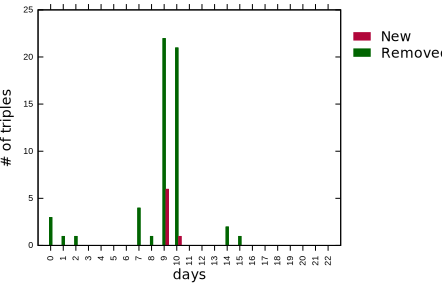
\includegraphics[width=0.8\textwidth]{images/updating_1.pdf}
  \end{center}
  \caption{Number of new coming soon movies, which are published on IMDb per day.}
  \label{fig_coming_soon_movie}
\end{figure}

From this observation we decided to update coming soon movies from IMDb daily.
Upcoming movies from the other data sources are updated weekly.
In this way, movies, which come from Freebase, TMDb or OFDb, can already be matched to a movie of IMDb.
%TODO muss nicht sein, wenn IMDb den film noch nicht hat. Auch ist das ja nicht zwingend notwendig oder? wir matchen doch immer mit allen schon vorhandenen
% --> Haben wir nie weiter beachtet. Müssen wir so schreiben, dass es plausible klingt

\subsubsection{Updating existing movies}
In Figure \ref{fig_new_movie} the number of changed triples of a new released movie from IMDb is displayed.
Therefor, a movie was crawled and triplified daily.
As you can seen, the movie frequently changes in the first days.
Also, the number of changing triples decreases with time.
Often changing triples are for example cast triple, links to images and videos, IMDb rating, charachter triples or taglines.

\begin{figure}[h!]
  \begin{center}
  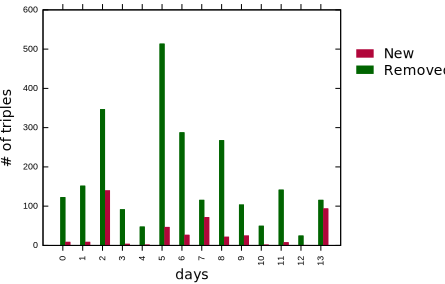
\includegraphics[width=0.8\textwidth]{images/updating_2.pdf}
  \end{center}
  \caption{Number of triples, which change in the first days of a new released movie from IMDb.}
  \label{fig_new_movie}
\end{figure}

Because a movie changes less the older the movie is, existings movies are divided into different categories.
Each category is updated at different frequencies (Table \ref{tab_updating_existing}).
\begin{table}[ht]
	\begin{center}
	\begin{tabular}{rl}
		\textbf{category of movie} & \textbf{frequency} \\ \hline
		one year old & weekly \\
		5 year old & monthly \\
		5 - 25 years old & yearly \\
		older than 25 years & never \\
	\end{tabular}
	\end{center}
	\caption{Frequency of updating existing movies}
	\label{tab_updating_existing}
\end{table}
If a category should be updated, the scheduler does the follwing steps:
\begin{enumerate}
	\item Find all movies, which should be updated regardless their originial data source.
	\item For each of these movies, get the updated movie resource and triplify it.
	\item Delete all triples of the movie in the triple store in the corresponding graph.
	\item Load the new triples into the corresponding graph in the triple store.
\end{enumerate}
Because the movies are stored in different graphs depending on their originial data source, the scheduler knows, where to find the movie resource in the web.
The originial resource of a movie is stored in a \emph{sameAs} triple.
Deleting the existing triples and storing the new downloaded triples, ensures that no conflicting information is stored of a resource.
\newpage
\section{Evaluation}
\label{sec_evaluation}

... some text ...

\subsection{Matching}
\label{subsec_evaluation_matching}
\subsection{Updating}
\label{subsec_evaluation_updating}

The scheduler, described in Chapter \ref{subsec_method_updating}, updates movies at certain times.
Thereby, the scheduler distinguish between existing and coming soon movies.

How many coming soon movies are daily added to IMDB is shown in Figure \ref{fig_coming_soon_movie}.
On a daily basis, the coming soon page from IMDB was crawled and the changes were recorded.
Almost every day, new movies are added or deleted from the IMDB coming soon list.
It is noticeable, that the most movies are published between Thursdays to Sundays on IMDB.

\begin{figure}[ht]
  \begin{center}
  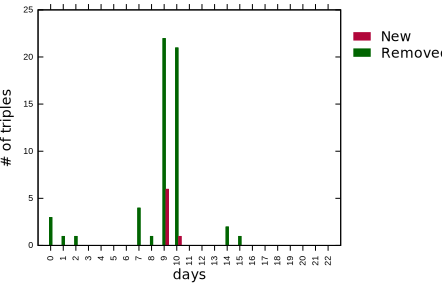
\includegraphics[width=0.5\textwidth]{images/updating_1.pdf}
  \end{center}
  \caption{Number of new coming soon movies, which are published on IMDB per day.}
  \label{fig_coming_soon_movie}
\end{figure}

In Figure \ref{fig_new_movie} the number of changed triples of a new released movie from IMDB is displayed.
Therefor, the movie was crawled and triplified daily.
As you can seen, the movie frequently changes in the first days.
Often changing triples are for example cast triple, links to images and videos, IMDB rating, charachter triples or taglines.

\begin{figure}[ht]
  \begin{center}
  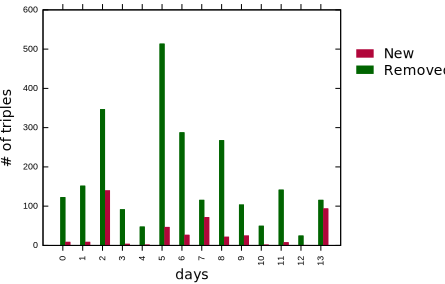
\includegraphics[width=0.5\textwidth]{images/updating_2.pdf}
  \end{center}
  \caption{Number of triples, which change in the first days of a new released movie from IMDB.}
  \label{fig_new_movie}
\end{figure}
\newpage
\section{Discussion}
\label{sec_discussion}

Outlook SMM Comparision

\newpage
%!TEX root = ../lod-group1.tex
\section{Conclusion and Outlook}
\label{sec_conclusion}

\emph{Match Forrest, Match!} is a system which combines various pieces of information from different data sources to a unified, linked open dataset of movies.
The system is based on the four online movie data sources IMDb, TMDb, OFDb and Freebase.
The paper detailed the resulting movie ontology and the system architecture.
Because a movie can exist in more than one of these data sources, a matching algorithm was developed and presented in this paper.
Thus, a movie appears only once in the resulting dataset.
Thereby, the focus was on a high precision to keep the merged data clean.
The developed matching algorithm was based on to steps: first candidate selection and then overlap scoring.
The candidate selection is fast and provides possible movie matches.
The overlap scoring is based on the ratio of actors starring in both movies and runs only on the selected candidates to keep the runtime low.

Overall, the algorithm has a high precision, while still maintaining a good recall.
Furthermore, a strategy to keep the resulting dataset up-to-date was explained in this paper.
The movies are divided into different categories depending on their age (time passed since they were published) and updated at different frequencies, because the older a movie gets, the less likely are changes.

In the future, the system could include more online movie databases.
For example, a data source which contains Indian movies would be useful to expand the number and range of movies.
Also, the system could be connected to DBpedia in the future, as DBpedia is the core of the Semantic Web.
Besides, the system could also include more resources than only feature movies, such as TV films or TV series.
Furthermore, it would be helpful for users who want to search for movies, only knowing some plot points, to build a website or an application which allows simple searching.
To increase the number of found matches, the matching algorithm could be improved further.
The most potential for that is in the candidate selection step.



%% Anhänge
\newpage
\begin{appendix}


%!TEX root = ../lod-group1.tex
%\section{Glossary} %Appendix (Glossar)


%\begin{description}
%\item[Browser:]\index{Browser} blabla
%\end{description}


%\newpage

% Appendix (Akronyme)
%\section{Abbreviations and Acronyms}\index{Acronyms}

%\begin{tabbing}
%\hspace*{3cm}\=  \\ \kill
%WWW \> World Wide Web\\
%\end{tabbing}

$N = \{$LotR\textsubscript{N}, FG\textsubscript{N}, GoT\textsubscript{N}, BB\textsubscript{N}, HP\textsubscript{N}$\}$

$M = \{$LotR\textsubscript{M}, FG\textsubscript{M}, HP\textsubscript{M}$\}$ \\

Matches returned by the system:

$\{
($LotR\textsubscript{N}, LotR\textsubscript{M}$);
($FG\textsubscript{N}, HP\textsubscript{M}$);
($GoT\textsubscript{N}, $\mathbf{\bot});
($BB\textsubscript{N}, HP\textsubscript{M}$);
($HP\textsubscript{N}, $\mathbf{\bot})
\}$

\begin{table}[h]
\begin{tabular}{|l|l|l|l|l|l|}
\hline
                       & \textbf{LotR\textsubscript{N}} & \textbf{FG\textsubscript{N}} & \textbf{GoT\textsubscript{N}} & \textbf{BB\textsubscript{N}} & \textbf{HP\textsubscript{N}} \\ \hline
\textbf{LotR\textsubscript{M}}  & TP                    & TN                  & TN                   & TN                   & TN                  \\ \hline
\textbf{FG\textsubscript{M}}    & TN                    & FN                  & TN                   & TN                   & TN                  \\ \hline
\textbf{HP\textsubscript{M}}    & TN                    & FP                  & TN                   & FP                   & FN                  \\ \hline
$\mathbf{\bot}$                 & TN                    & TN                  & TN                   & TN                   & TN                  \\ \hline
\end{tabular}
\end{table}

\section{Exact Results for Evaluation of the Matching}

\label{appendix_data}

\begin{table}[h!]
\centering
\begin{tabular}{l|l|l|l}
\multicolumn{1}{c|}{\bfseries $CANDIDATE_\_SET\_SIZE$} & \multicolumn{1}{|c|}{\bfseries Precision} & \multicolumn{1}{|c|}{\bfseries Recall} & \multicolumn{1}{|c}{\bfseries F0.5}
\\ \hline \hline
%\endhead


2    & 0.977246871445 & 0.855577689243 & 0.950221238938 \\ \hline
4    & 0.975355969332 & 0.886952191235 & 0.956292955326 \\ \hline
8    & 0.974040021633 & 0.896912350598 & 0.957571246278 \\ \hline
16   & 0.973584905660 & 0.899402390438 & 0.957685320322 \\ \hline
32   & 0.973103819258 & 0.900896414343 & 0.957750952986 \\ \hline
64   & 0.971535982814 & 0.900896414343 & 0.956535532995 \\ \hline
128  & 0.968415417559 & 0.900896414343 & 0.954113924051 \\ \hline
256  & 0.966382070438 & 0.901892430279 & 0.952756734007 \\ \hline
512  & 0.960742705570 & 0.901892430279 & 0.948366149979 \\ \hline
1024 & 0.955168776371 & 0.901892430279 & 0.944015846539 \\ \hline
2048 & 0.950656167979 & 0.901892430279 & 0.940486082260 \\ \hline
4096 & 0.949161425576 & 0.901892430279 & 0.939315352697 \\ \hline

\end{tabular}
\caption{Parameter optimization for the optimal candidate set size.}
\end{table}
 

\begin{longtable}{l|l|l|l|l}
\multicolumn{1}{c|}{\bfseries $MIN\_SCORE$} & \multicolumn{1}{|c|}{\bfseries $ACT\_DIST$} & \multicolumn{1}{|c|}{\bfseries Precision} & \multicolumn{1}{|c|}{\bfseries Recall} & \multicolumn{1}{|c}{\bfseries F0.5}\\ \hline
\endhead
 \hline


\multirow{4}{*}{0.1} & 1 & 0.9938340807 & 0.8829681275 & 0.9694881890 \\ \hhline{~----}
					 & 2 & 0.9938340807 & 0.8829681275 & 0.9694881890 \\ \hhline{~----}
					 & 3 & 0.9916154276 & 0.8834661355 & 0.9679179398 \\ \hhline{~----}
					 & 4 & 0.9833610649 & 0.8829681275 & 0.9614967462 \\ \hline
 \hline
\multirow{4}{*}{0.2} & 1 & 0.9949409781 & 0.8814741036 & 0.9699693117 \\ \hhline{~----}
					 & 2 & 0.9949494949 & 0.8829681275 & 0.9703371278 \\ \hhline{~----}
					 & 3 & 0.9943946188 & 0.8834661355 & 0.9700349956 \\ \hhline{~----}
					 & 4 & 0.9910564561 & 0.8829681275 & 0.9673723265 \\ \hline
 \hline
\multirow{4}{*}{0.3} & 1 & 0.9954827781 & 0.8779880478 & 0.9695336560 \\ \hhline{~----}
					 & 2 & 0.9954878737 & 0.8789840637 & 0.9697802198 \\ \hhline{~----}
					 & 3 & 0.9954929577 & 0.8799800797 & 0.9700263505 \\ \hhline{~----}
					 & 4 & 0.9932659933 & 0.8814741036 & 0.9686952715 \\ \hline
 \hline
\multirow{4}{*}{0.4} & 1 & 0.9954622802 & 0.8740039841 & 0.9685430464 \\ \hhline{~----}
					 & 2 & 0.9954751131 & 0.8764940239 & 0.9691629956 \\ \hhline{~----}
					 & 3 & 0.9954802260 & 0.8774900398 & 0.9694102113 \\ \hhline{~----}
					 & 4 & 0.9943661972 & 0.8789840637 & 0.9689284146 \\ \hline
 \hline
\multirow{4}{*}{0.5} & 1 & 0.9959977130 & 0.8675298805 & 0.9673478454 \\ \hhline{~----}
					 & 2 & 0.9954493743 & 0.8715139442 & 0.9679203540 \\ \hhline{~----}
					 & 3 & 0.9954571266 & 0.8730079681 & 0.9682942996 \\ \hhline{~----}
					 & 4 & 0.9954674221 & 0.875        & 0.9687913542 \\ \hline
 \hline
\multirow{4}{*}{0.6} & 1 & 0.9728531856 & 0.8745019920 & 0.9514521023 \\ \hhline{~----}
					 & 2 & 0.9725274725 & 0.8814741036 & 0.9528423773 \\ \hhline{~----}
					 & 3 & 0.9726477024 & 0.8854581673 & 0.9538626609 \\ \hhline{~----}
					 & 4 & 0.9727223131 & 0.8879482071 & 0.9544967880 \\ \hline
 \hline
\multirow{4}{*}{0.7} & 1 & 0.9964264443 & 0.8331673307 & 0.9588491518 \\ \hhline{~----}
					 & 2 & 0.9958920188 & 0.8451195219 & 0.9615820490 \\ \hhline{~----}
					 & 3 & 0.9959159860 & 0.8500996016 & 0.9628835740 \\ \hhline{~----}
					 & 4 & 0.9959325973 & 0.8535856574 & 0.9637876743 \\ \hline

\caption{Results for the optimization of the actor Levenshtein distance and minimal score parameter.}
\label{tab_overlapScore}
\end{longtable}



\begin{table}[h!]
\centering
\begin{tabular}{l||l|l|l}
 &  \multicolumn{1}{|c|}{\bfseries Precision} &  \multicolumn{1}{|c|}{\bfseries Recall} &  \multicolumn{1}{|c}{\bfseries F0.5}
\\ \hline \hline
%\endhead

\textbf{Baseline}       & 0.5923566878980892 & 0.5925663716814159 & 0.592398612782221 \\ \hline
\textbf{MFM with id}    & 0.991807755324959 & 0.88671875 & 0.9688433632095604 \\ \hline
\textbf{MFM without id} & 0.8928571429 & 0.7142857143 & 0.8503401361 \\

\end{tabular}
\caption{Final evaluation results comparing Baseline and the MFM approach.}
\end{table}

%precision_baseline,precision_mfm_with_id,precision_mfm_without_id,recall_baseline,recall_mfm_with_id,recall_mfm_without_id,f0.5_baseline,f0.5_mfm_with_id,f0.5_mfm_without_id
%0.5923566878980892,0.991807755324959,0.8928571429,0.5925663716814159,0.88671875,0.7142857143,0.592398612782221,0.9688433632095604,0.8503401361


\end{appendix}


%Hier kommt das Literaturverzeichnis
\newpage

\addcontentsline{toc}{section}{References} % Zeile für das Inhaltsverzeichnis

\bibliography{bibfile}
\bibliographystyle{alphadin}

\newpage

%Hierhin kommt der Index (Sachverzeichnis)
%\addcontentsline{toc}{section}{Index} % Dies ist die Zeile für das Inhaltsverzeichnis
%\flushbottom
%\printindex

\end{document}
